

\documentclass[oneside,20pt]{article}          % please do not change
\usepackage[b5paper]{geometry}	    % your paper can be easily printed on a4 or letter paper with enlargenment      
                                    % comment if you have problem with print     
\usepackage{amsfonts,amsmath,latexsym,amssymb}
\usepackage{graphicx}
%%% remove comment delimiter ('%') and specify parameters if required
%\usepackage[dvips]{graphics}

\begin{document}

%%% remove comment delimiter ('%') and select language if required
%\selectlanguage{spanish} 

\noindent 
\begin{center}
  \texttt{LABORATOR 1-- Application Hacking cu Python.}        
\end{center}

\section{Introducere}
\noindent                 
\\\\\
Pentru a pirata o aplicație Windows folosind Python, este necesar
pentru a avea cunoștințe de bază despre API-ul Windows. API Windows
constă dintr-un set de interfețe de programare a aplicațiilor (API)
furnizate de Microsoft. Pentru a dezvolta o aplicație folosind
Windows API, este necesar să utilizați diverse funcții care sunt
suportate de sistemul de operare (kernel). Pentru utilizare în mod obișnuit Mediu Windows pe 32 de biți, API-ul Windows numit Win32 API este suportat.
  \begin{center}
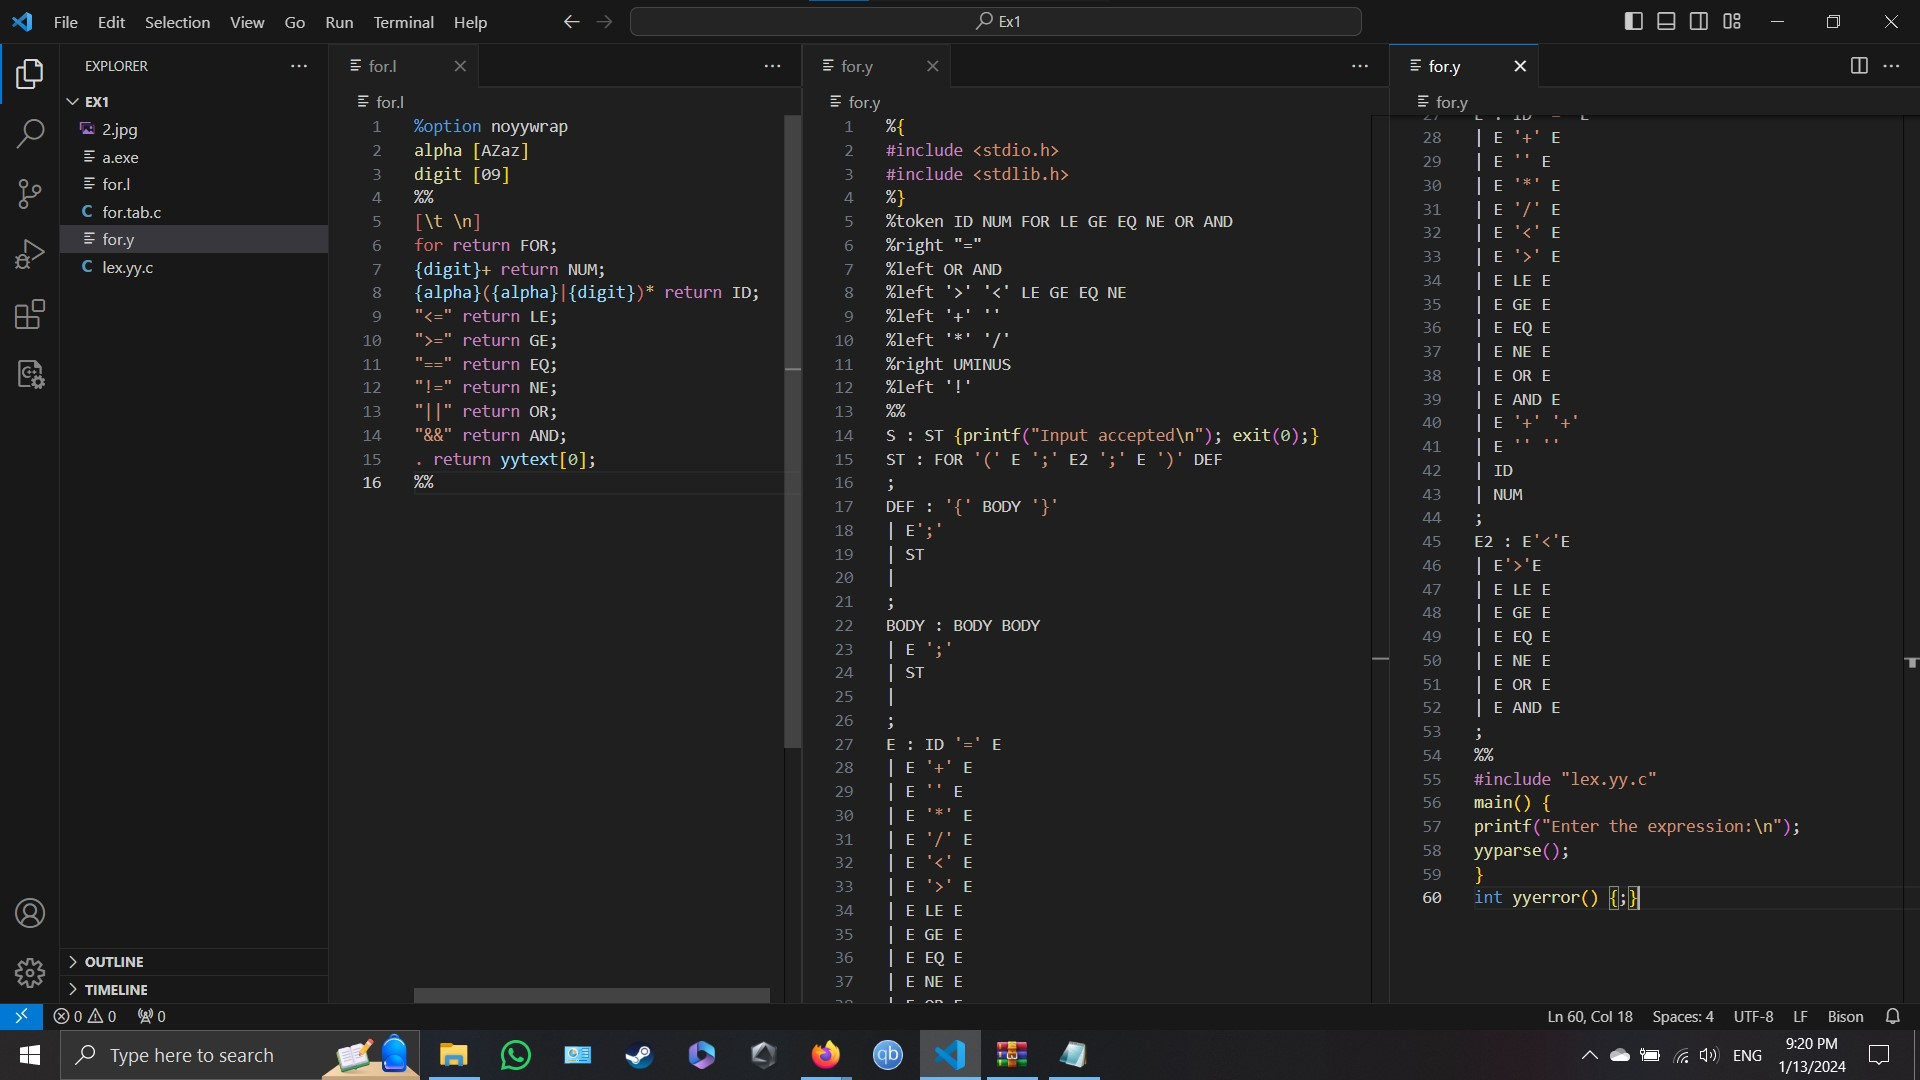
\includegraphics[height=5 cm]{1.png}
\end{center}
Folosim biblioteci precum ”lib” și ”DLL” atunci când o aplicație Windows este
dezvoltată. ”Lib” este o bibliotecă statică care este inclusă atunci când 
este creat fișierul executabil Windows. ”DLL” (dynamical lynked library) oferă o bibliotecă dinamică care este apelată în timpul
execuției aplicației. Putem folosi la maximum Win32 API sub formă de DLL, unde sunt de obicei următoarele DLL-uri
sunt folosite:
 \begin{center}
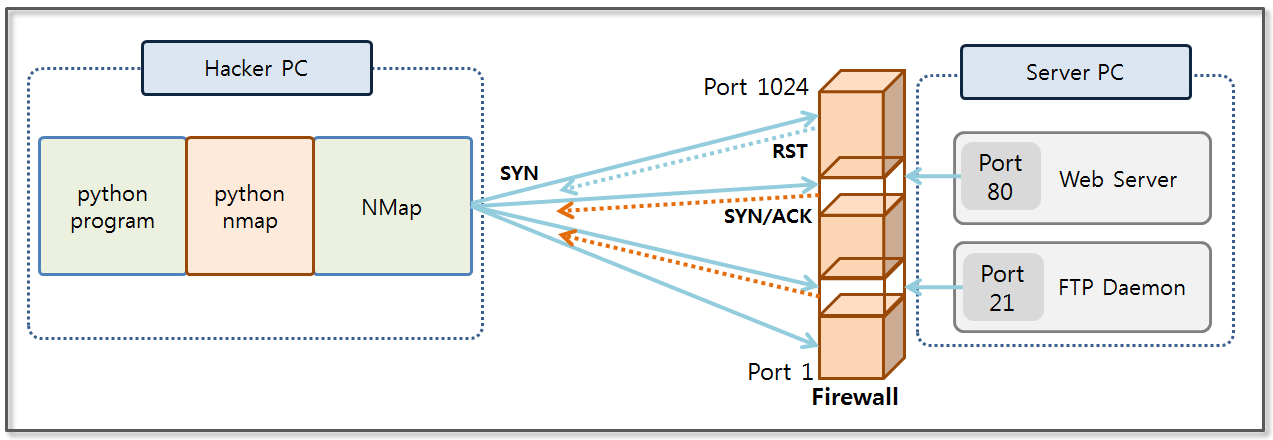
\includegraphics[height=10 cm]{2.png}
\end{center}
Exemplu de biblioteca externa folosita de python:
\begin{center}
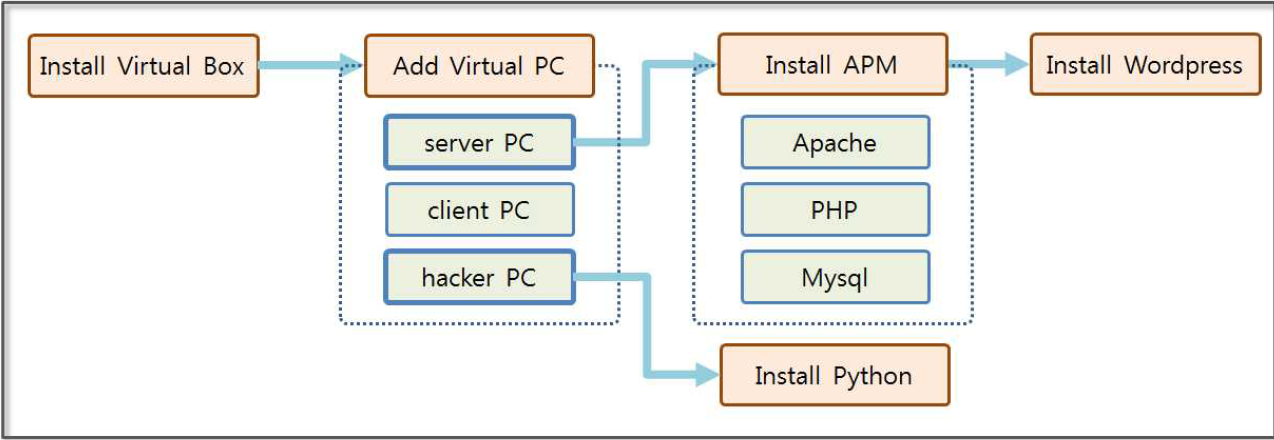
\includegraphics[height=5 cm]{3.png}
\end{center}
La început, atunci când utilizați API-ul Win32 și ctypes, poate fi dificil de utilizat apelurile API Win32 prin utilizarea ctypes. Există
o cantitate extinsă de cunoștințe care este necesară în prealabil, de exemplu
un mecanism de apelare a funcției, valori returnate și tipuri de date.
Cu toate acestea, ctypes pot fi folosite pentru biblioteci native care sunt
susținute de o varietate de sisteme de operare, care oferă o unealtă puternică. Pentru a implementa tehnici sofisticate de hacking,
ar trebui înțeles conceptul de bază al c-tipurilor (ctypes).
 C-typeurile simplifică procedura de a efectua apeluri dinamice de biblioteci,
iar acestea suportă tipuri complexe de date in C și au avantajul
oferind funcționalitate de nivel scăzut. Dacă respectați convențiile la
apelarea funcțiilor pentru a profita de ctypes, puteți apela API-ul
care este furnizat direct de MSDN.
Conceptul de baza a unui Ctype se poate obseva mai jos
\begin{center}
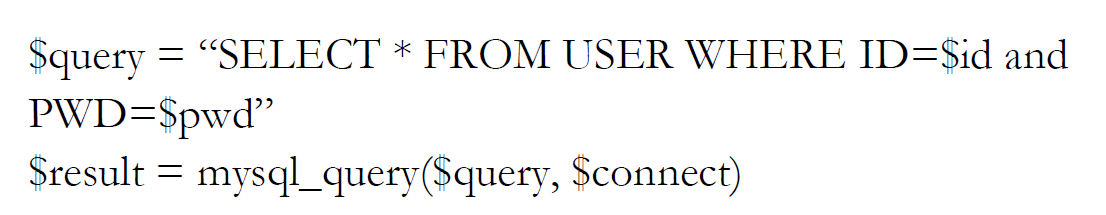
\includegraphics[height=5 cm]{4.png}
\end{center}
\section{Funcții in Python}
Ca și în cazul altor limbaje, Python folosește funcții pentru a fi îmbunătățit structural și pentru a elimina codul duplicat. Python suportă
o varietate de funcții încorporate care pot fi utilizate prin includerea a
unui apel de funcție sau importul unui modul. Cel mai frecvent utilizată  este funcția ”print” și poate fi folosită fără instrucțiuni de import, dar
funcțiile matematice pot fi utilizate numai după importarea  modulului ”math”. 
\begin{center}
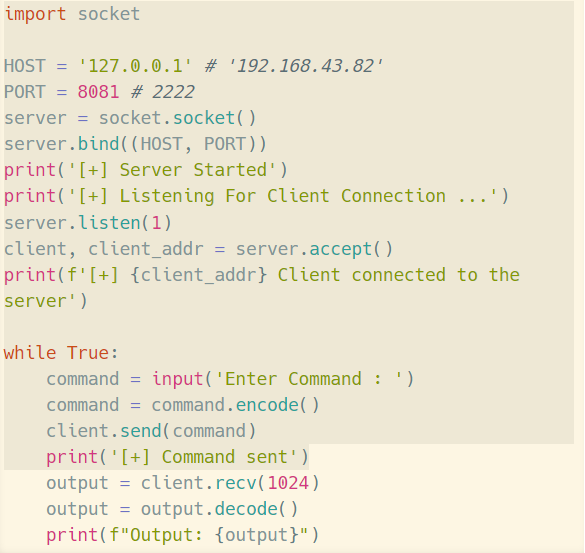
\includegraphics[height=2 cm]{5.png}
\end{center}
Este posibil să dezvoltam programe cu Python atât în ​​
mod procedural cat şi orientat pe obiecte. Pentru a dezvolta simplu
programe de hacking, este convenabil să folosiți o manieră procedurală.
Cu toate acestea, pentru a dezvolta programe complexe care sunt necesare pentru
funcționarea într-un mediu diferit, este necesară structurarea
programului. Un limbaj orientat pe obiect poate fi folosit pentru a îmbunătăți
productivitatea în timpul dezvoltării permițând reutilizarea. Dacă utilizați un limbaj orientat pe obiecte, este posibil
a dezvolta un program care este construit logic.
Structura de bază pentru declararea unei clase este următoarea.
\begin{center}
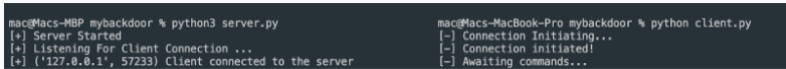
\includegraphics[height=2 cm]{6.png}
\end{center}

\textbf{(1) Creați o clasă}: dacă specificați un nume de clasă după ce ați folosit cuvânt rezervat ”clasă”, clasa este declarată.\\
\textbf{(2) Constructor}: Funcția ”init” este un constructor care este
apelat implicit atunci când clasa este creată.\\
\textbf{(3) Funcție}: Este posibil să se declare o funcție în clasă. O
instanța este apoi generată pentru a apela funcția.
\textbf{(4) Moștenire}: Pentru a moșteni dintr-o altă clasă un nume, numele de
clasa moştenită trebuie folosită ca argument când clasa
este declarată. Moștenirea acceptă utilizarea variabilelor membre și funcțiile clasei superioare așa cum sunt.
\section{Crearea unei clase:}
\begin{center}
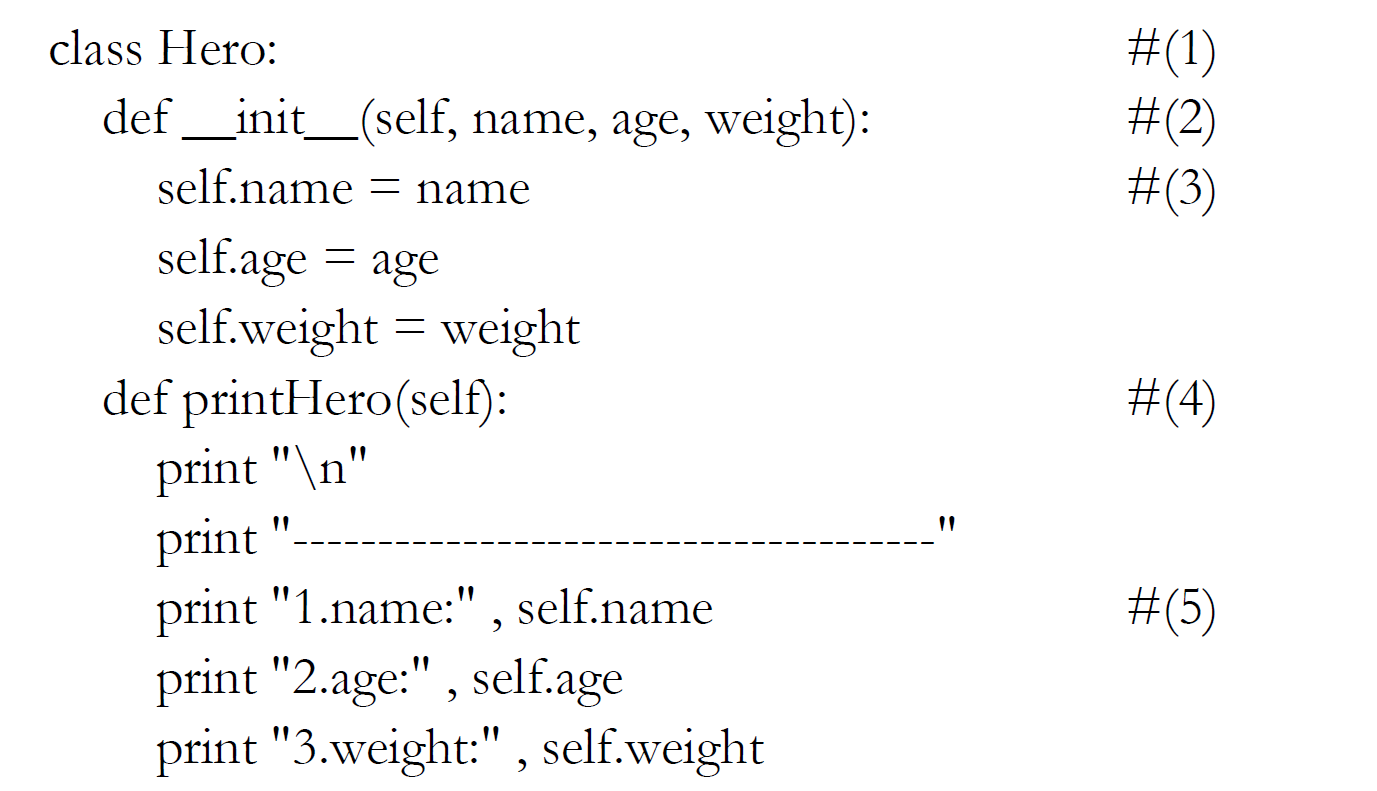
\includegraphics[height=4 cm]{7.png}
\end{center}
\begin{center}
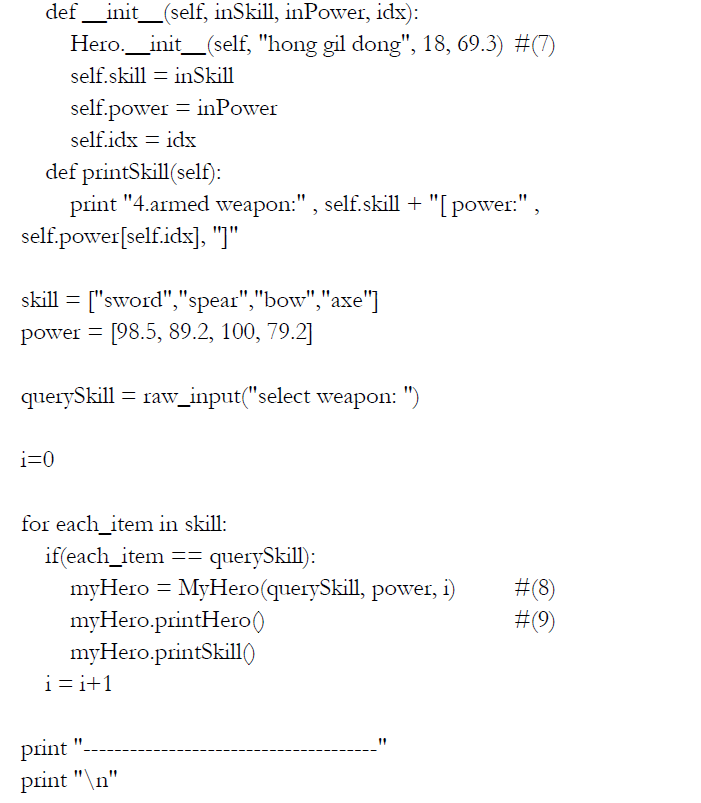
\includegraphics[height=8 cm]{8.png}
\end{center}
Aici avem:\\
(1) Declarație de clasă: Declarați clasa ”Hero”.\\
(2) Declarația constructorului: Declarați constructorul care ia trei argumente și ”self” reprezentând clasa în sine.\\
(3) Inițializarea variabilelor: Inițializați variabilele clasei prin atribuirea argumentelor.\\
(4) Declarație de funcție: Declarați funcția ”printHero” în clasa.\\
(5) Utilizarea variabilelor: Folosiți variabile de clasă în formatul de
”self.nume variabilă”.\\
(6) Moștenirea clasei: Declarați clasa ”MyHero” care moștenește
clasa ”Erou”.\\
(7) Apelarea constructorului: Generați și inițializați obiectul prin
apelând constructorul clasei superioare.\\
(8) Crearea unei clase: Generați o clasă ”MyHero”. Treceți argumentele cerute constructorului.\\
(9) Funcția de clasă de apelare: sarcinile sunt executate prin apelarea funcțiilor care sunt declarate pentru obiectul ”myHero”.\\
\section{Șiruri în Python (String)}
Formatul șir este o tehnică care poate fi folosită pentru a introduce un anumit
valoare în șirul pe care doriți să-l imprimați. Tipul valorii
inserat este determinat de un cod de format șir. Formatul șirului este folosit în felul următor.

$$ print(output\; string1\; \%s\; output string2\; \%\; inserted\; string)$$
Introduceți codul formatului șirului în mijlocul șirului de ieșire.
Puneți caracterele pe care doriți să le introduceți cu simbolul $\% $ după
șir.
Codurile de formatare a unui șir în Python:
\begin{center}
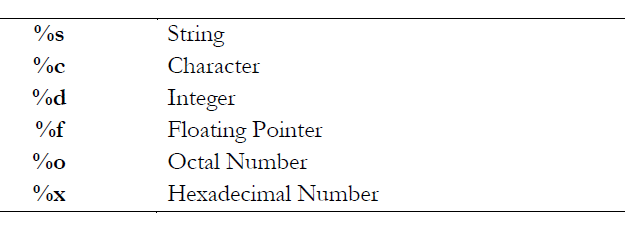
\includegraphics[height=3 cm]{9.png}
\end{center}
Putem observa formatarea unui șir în Python prin exemplul următor:

\begin{center}
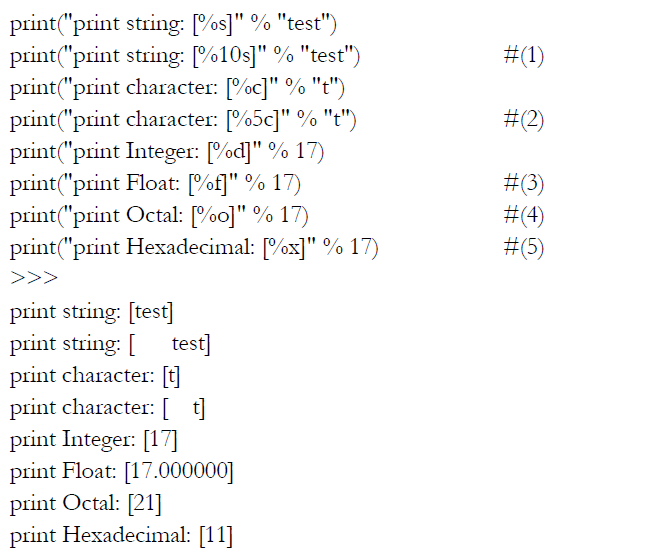
\includegraphics[height=5 cm]{10.png}
\end{center}
Dacă utilizați codurile de formatare a șirurilor și numerele împreună,
caracterele pot fi folosite pentru a asigura un spațiu în funcție de dimensiunea
numerelor care sunt printate pe ecran.
(1) Imprimarea unui șir de caractere cu lungime fixă: dacă se folosește $\%s$.
cu un număr, se asigură spațiul cu o sumă corespunzătoare numarul. În exemplu, test este tipărit folosind 4 cifre și
spațiile sunt tipărite pentru celelalte șase cifre, deci toate cele 10 caractere sunt tipărite.\\
(2) Imprimarea unui caracter fix care conține spații de o anumita Lungime: Dacă $\%c$ este folosit cu un număr, suma
corespunzătoare numărului care este aceeasi ca pentru $\%s$.\\
Prin urmare, sunt imprimate un caracter și patru spații libere.\\
(3) Șirul este același cu cel folosit cu numărul $\%c$,
care poate fi extras numai ca număr. Din caracterul lui este extras un spațiu liber de 4 cifre.\\
(3) Număr real: 17 este convertit într-un număr real.\\
(4) Octal: 17 este convertit într-un număr octal, iar 21 este printat.\\
(5) Hexazecimal: 17 este convertit într-un număr hexazecimal, iar 11 este printat.\\

\section{Spargerea unei parole cu Python}
Spargerea unei parole NU este etică și reprezinta o Infracțiune informatică. Prezentăm doar în scop EDUCAȚIONAL (în Python) acest aspect.
În cele ce urmeaza, vom programa in Python pentru a sparge parola unui fișier zip folosind metoda forței brute.

Formatul de fișier ZIP este un standard comun de arhivă și compresie. Este folosit pentru a comprima fișiere. Uneori, fișierele comprimate sunt confidențiale și proprietarul nu dorește să ofere acces fiecărui individ. Prin urmare, fișierul zip este protejat cu o parolă. Dacă parola este obișnuită, atunci este ușor de spart. Aici, vom folosi metoda forței brute pentru a sparge parola fișierului zip.\\

Cum să forțați parolele fișierelor ZIP în Python?\\
O metodă de forță brută este o metodă în care un set de valori predefinite sunt folosite pentru a sparge o parolă până la succes. Aceasta este practic o metodă de ”loviți și încercați”. Această metodă poate dura mult timp dacă setul de valori este mare, dar rata de succes este mare. Cu cât numărul de valori este mai mare, cu atât sunt mai mari șansele de spargere a parolelor. Aici vom folosi fișierul text ”rockyou”, cu cateva parole de încercat.

Abordare:  

Mai întâi, importați modulul zipfile.\\
Inițializați obiectul ZipFile care ajută la extragerea conținutului fișierului zip.\\
Numărați numărul de cuvinte prezente în fișierul „rockyou.txt” și afișați-l pe terminal.\\
Apelați funcția crack password care returnează adevărat dacă este găsită o parolă, altfel returnează false. Treceți numele fișierului text și obiectul ZipFile ca parametri.\\
Variabila idx este folosită pentru a ține evidența numerelor de linii.
Deschideți fișierul text rockyou.txt în modul rb pentru a gestiona conținutul fișierului în formă binară. Acest lucru se datorează faptului că fișierul conține unele simboluri speciale care nu pot fi gestionate dacă fișierul este deschis în modul r și va genera UnicodeDecodeError.
După deschiderea fișierului, extrageți linia din fișier și apoi împărțiți cuvântul din acesta.
În blocul try, extrageți conținutul fișierului zip dând parola către câmpul pwd al metodei extractall. Metoda extractall() va extrage tot conținutul fișierului zip în directorul de lucru curent. Programul de mai sus extrage un fișier zip numit gfg.zip în același director cu acest script Python.
Dacă parola este incorectă, va fi generată o excepție. În except block, continuați bucla pentru a verifica alte cuvinte din fișier.
Dacă parola este găsită, returnează adevărat, altfel returnează false și afișează mesajul dorit.\\ 
A se implementa la laborator.
\begin{center}

\includegraphics[height=5 cm]{11.png}
\end{center}


\section{Concluzie}
În acest laborator, am explicat cateva concepte de baza pentru Python si cum poate fi folosit pentru aplicatii de piratare -ceea ce POATE sa reprezinte o mare vulnerabilitate a PC-urilor.

Nu utilizați aceste informatii pentru a obține acces nedorit la orice computer fără permisiune, deoarece este \textbf{ilegal}. Nu utilizați Python pentru infractiuni informatice deoarece este Ilegal!\\

Pentru bibliografie mai detaliata lecturati capitolul I din cartea de mai jos:
\section{Bibliografie}

Python Hacking Essentials Paperback 2015 by Earnest Wish, \\
https://www.amazon.com/Python-Hacking-Essentials-Earnest-Wish/dp/1511797568


\end{document}
